\section{Auswertung}
\label{sec:evaluation}
Ausgleichsrechnungen mit den dazugehörigen Fehlern werden mit dem \texttt{python}-Paket \texttt{SciPy} \cite{scipy} erstellt, weitere Fehler werden mit dem \texttt{python}-Paket \texttt{uncertainties} \cite{uncertain} berechnet, welches eine automatische Gauß'sche Fehlerfortpflanzung bereitstellt.

\subsection{Frequenzgang eines gegengekoppelten Verstärkers}
\label{Frequenzgang}
Die Frequenzabhängigkeit des Linearverstärkers wird untersucht, indem die Verstärkung bei verschiedenen Frequenzen über mehrere Zehnerpotenzen gemessen wird. Dies wird für vier verschiedene Kombinationen von Widerständen durchgeführt. Eine doppelt-logarithmische Darstellung der Frequenzgänge ist in \autoref{loglog-plot} gezeigt. Die durchgezogene Linie stellt dabei jeweils den linearen Fit der Form
\begin{equation}
	\log_{10} V^\prime = A \cdot \log_{10} \nu + B
	\label{linear_fit}
\end{equation}
an den abfallenden Teil bei hohen Frequenzen dar, wobei $V^\prime = U_\text{A} / U_\text{E}$ ist. In \autoref{a} werden die verwendeten Widerstände, die daraus resultierenden Fitparameter und die Grenzfrequenzen -- also die Frequenz, bei der die Verstärkung auf $V'/\sqrt{2}$ abgefallen ist -- zusammengefasst. Das Verstärkung-Bandbreite-Produkt $\nu_\text{G}V^\prime$ ist ebenfalls eingetragen. Der Mittelwert des Verstärkung-Bandbreite-Produkts der vier gemessenen Widerstandskombinationen ist $\SI{833 \pm 37}{\hertz}$, die Abweichungen der einzelnen Werte vom Mittelwert liegen zwischen 1.6\% und 6.6\%.\par
Mit \autoref{effVerstaerkung} kann aus $V^\prime$ und den beiden Widerständen $R_1$ und $R_\text{N}$ die Leerlaufverstärkung $V$ mit
\begin{equation}
	V = \frac{R_\text{N} + R_1}{\frac{R_\text{N}}{V^\prime} - R_1}
\end{equation}
abgeschätzt werden. Die entsprechenden Werte sind ebenfalls in \autoref{a} eingetragen.

\begin{figure}[h]
	\centering
	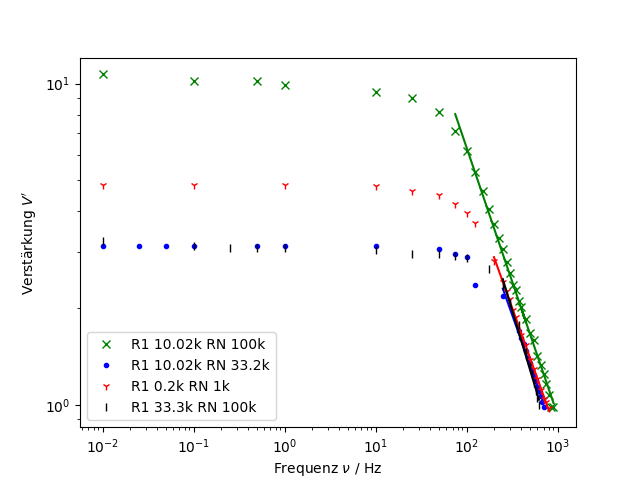
\includegraphics[width=\textwidth]{img/a.png}
	\caption{Frequenzgang eines gegengekoppelten Verstärkers - bei kleinen Frequenzen ist die Verstärkung in etwa konstant, nimmt dann aber mit größer werdenden Frequenzen exponentiell ab.}
	\label{loglog-plot}
\end{figure}

\begin{table}[h]
	\caption{blub}
	\label{a}
	\centering
	\begin{tabular}{ccccccccc}
		$R_1/\si{\kilo\ohm}$	&	$R_\text{N}/\si{\kilo\ohm}$	&	A	&	B	&	$V^\prime$	&	$R_{N}/R_1$	&	$\nu_\text{G}/\si{\hertz}$	&	$\nu_\text{G}V^\prime/\si{\hertz}$	&	$V$	\\ \toprule
		10.02	&	100.0	&	-0.83\pm0.01	&	2.47\pm0.03	&	10.69 	&	9.98	&	80.74	&	862	&	-165.33\\
		10.02	&	33.2	&	-0.80\pm0.02	&	2.27\pm0.06	&	3.13 	&	3.31	&	262.07	&	820	&	226.91\\
		0.20	&	1.0	&	-0.79\pm0.01	&	2.28\pm0.03	&	4.85 	&	5.00	&	160.60	&	778	&	194.00\\
		33.30	&	100.0	&	-0.94\pm0.04	&	2.70\pm0.10	&	3.25 	&	3.00	&	269.00	&	873	&	-52.67\\
	\end{tabular}
\end{table}

\FloatBarrier

\subsection{Umkehr-Integrator}

\FloatBarrier

\subsection{Umkehr-Differentiator}

\FloatBarrier

\subsection{Schmitt-Trigger}

\FloatBarrier

\subsection{Beziehung zwischen Frequenz und Phase}

Die Phase zwischen Eingangs- und Ausgangsspannung in Abhängigkeit von der Frequenz hat einen ähnlichen Verlauf, wie die Verstärkung, sie ist in \autoref{Phasenbeziehung}. Zunächst ist die Phase konstant und nahezu $180^\circ$. Nach einer Frequenz von \SI{10}{\hertz} fällt die die Phase ab. Das ist mit dem Einsetzen des Tiefpass-Verhaltens des Operationsverstärkers zu erklären; bei hohen Frequenzen sinkt die Verstärkung auf 1 ab. Die Übertragungsfunktion eines Tiefpasses verläuft gemäß
\begin{equation}
	H(\omega) = \frac{1}{1 + i\frac{\omega}{\omega_\text{g}}},
\end{equation}
das heißt, je näher die Frequenz gegen die Grenzfrequenz $\omega_\text{g}$ geht, desto größer ist die Phasendrehung. Der Phasengang eines Operationsverstärkers folgt nicht dem Verlauf eines reinen Tiefpasses, sondern ist abhängig vom Inneren Aufbau, tendentiell lässt sich aber sagen, dass auch hier die Phasendrehung mit größerer Frequenz steigt.

\begin{figure}[h]
	\centering
	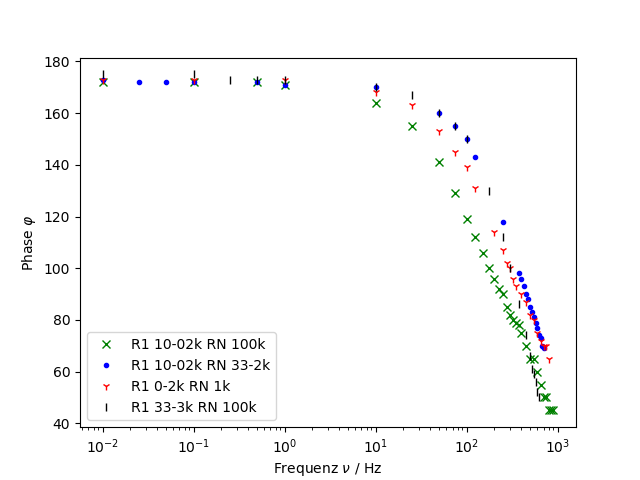
\includegraphics[width=\textwidth]{img/j.png}
	\caption{Bis zu einer Frequenz von \SI{10}{\hertz} ist die Phase relativ konstant bei knapp $180^\circ$, danach fällt sie in der halblogarithmischen Darstellung nahezu linear ab.}
	\label{Phasenbeziehung}
\end{figure}

\FloatBarrier
